\chapter{Estimación de las Condiciones Operativas de la Estación Remota}

Este capítulo tiene como objetivo considerar las condiciones térmicas de la Estación Remota, dentro de su contexto operativo en Palo Verde, se toma en cuenta su interrelación con el radio transmisor y el exterior que lo rodea, para lo cual se analizarán las condiciones conocidas respecto a la ubicación futura de la estación y se unificarán nuevamente en un modelo térmico, que no solo incluya el modelo térmico del radio, sino que a su vez contemple características físicas propias de la estación y del medio en que se encuentra, de manera tal que permita tomar la mejor ruta de acción en el planteamiento de una solución.

\section{Condiciones Generales de la Estación}

\subsection{Ubicación Exacta:}

Como ya antes se mencionó, la GRT estará ubicada en el Sitio Ramsar Parque Nacional Palo Verde. El parque se encuentra aproximadamente 30 kilómetros al oeste de la ciudad de Cañas, entre el Río Bebedero y el Río Tempisque,  es un área protegida con una extensión de 16804 hectáreas y fue creada bajo el decreto ejecutivo N0.11541 el 30 de mayo de 1980 y fue ratificado por la Ley No. 6831 del 20 de diciembre de 1982. \cite{paloverde}

En la Tabla \ref{cordenadas} se muestran datos sobre la ubicación específica de la torre donde se colocará  el gabinete que contiene la GRT. Por otra parte en  la Figura \ref{ubicacion} se muestra la imagen satelital de la ubicación actual de la torre.

\begin{table}[H]
\centering
\caption{Datos de la ubicación del gabinete}
\label{cordenadas}
\begin{tabular}{cc}
\toprule
Latitud (DMS) &  10\degree20'38.2"N \\
Longitud (DMS) & 85\degree20'17.1"W \\
Altura (msnm) & 10\\
Presión Atmosférica promedio (mbar) & 1006 \\ \bottomrule
\end{tabular}
\end{table}

\begin{figure}[H]
\centering
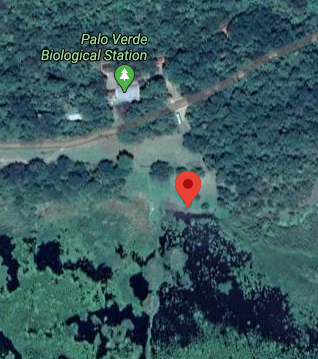
\includegraphics[scale=0.9]{Figuras/ubicacion_3.png}
\caption{Imagen Satelital de la posición de la GRT}
Fuente: Google Maps
\label{ubicacion}
\end{figure}

\subsection{Características físico-mecánicas del gabinete}

Para el montaje de los componentes internos de la GRT se hará uso de un gabinete metálico comercial, utilizado para montajes eléctricos de pared. Sus características principales se presentan en la Tabla \ref{gabinete},\cite{gabinete manual}.

\begin{table}[H]
\centering
\caption{Características del gabinete a utilizar en la GRT}
\label{gabinete}
%\begin{tabularx}{14cm}{l X}
\begin{tabular}{cc}
\toprule
\textbf{Fabricante}        & Hoffman                 \\
\textbf{Modelo}            & M600400225G             \\
\textbf{Dimensiones}       & (600x400x225) \si{\milli\meter}      \\
\textbf{Espesor de lámina} & \SI{1,2}{\milli\meter}                 \\
\textbf{Acabado} & \begin{tabular}[c]{@{}c@{}}Color Gris Claro RAL 7035 texturizado,\\ pintura poliéster en polvo por ambos lados\end{tabular} \\
\textbf{Certificaciones}   & IEC IP66 y UL Tipo 12/4 \\ \bottomrule
\end{tabular}
\end{table}

En la Figura \ref{gabinete1} se muestra un render realizado del gabinete real.

\begin{figure}[H]
\centering
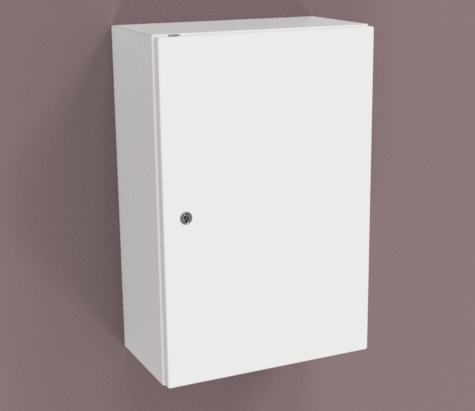
\includegraphics[scale=0.65]{Figuras/gabinete1.png}
\caption{Render del Gabinete Real}
Fuente: Elaboración Propia
\label{gabinete1}
\end{figure}

\section{Datos Meteorológicos}

Parte fundamental del modelo de la GRT implica conocer las condiciones de temperatura, radiación, dirección y velocidad del viento, que se requieren para la determinación de los diferentes parámetros termodinámicos de la simulación; para lo cual se utilizaron los datos de una estación meteorológica ubicada en la torre antes mencionada. Dichos datos eran accesibles al público a través de la OTS (\textit{Organization for Tropical Studies})\cite{ots}. Para todos los casos se recopilaron los datos de un año, comprendido entre el 1 de junio de 2019 al 1 de junio de 2020.

Los datos recopilados de la estación meteorológica, comprenden los promedios de mediciones realizadas cada 10 segundos en períodos de 15 minutos, de donde también se obtienen los valores máximos y mínimos de esos períodos de tiempo. \cite{ots}

\subsection{Temperatura}

Los datos de temperatura se organizaron en los valores correspondientes al día y los datos correspondientes a la noche, esto para no afectar el valor promedio anual de temperatura del aire, ya que para efectos del modelo es conveniente tener el valor promedio de temperatura del día, donde se espera que los valores típicos sean mayores que durante la noche.

En el caso de la resolución las regulaciones OMM (\textit{Organización Mundial de Meteorología}), indica que deben ser de \SI{0,1}{\celsius} y con una exactitud en los datos de \SI{0,2}{\celsius} , para una medición de temperatura a 1,5 metros del suelo. \cite{ots_manual}

En la Tabla \ref{temperatura_met} se muestran los datos obtenidos de la estación meteorológica para el período establecido.

\begin{table}[H]
\centering
\caption{Datos de Temperatura para el período entre 1/6/2019 y 1/6/2020}
\label{temperatura_met}
%\begin{tabularx}{12.5cm}{cccc}
\begin{tabular}{cccc}
\toprule
\multicolumn{1}{c}{\multirow{2}{*}{\textbf{Temperatura del Aire}}} & \multicolumn{3}{c}{\textbf{Valores de temperatura (\si{\celsius})}}           \\ \cline{2-4} 
\multicolumn{1}{c}{}                                & \textbf{Promedio} & \textbf{Valor máximo} & \textbf{Valor Mínimo} \\ \hline
Diurna         & 30,06 & 37,94 & 21,60 \\
Nocturna     & 26,46 & 33,88 & 21,46 \\
Día completo & 29,75 & 37,94 & 21,46 \\ \bottomrule
\end{tabular}
\end{table}

\subsection{Velocidad y Dirección del Viento}

La OMM indica que esta variable hace referencia a la velocidad del viento en superficie y para efectos meteorológicos es una cantidad vectorial compuesta por su dirección y magnitud. Su dirección se representa en grados dextrórsum, es decir en sentidos de las agujas del reloj, donde el Norte esta representado por los grados 0 y 360 y el grado 90 representa el Este. Para este caso la resolución de los datos es de 10 grados para la dirección y de 0,5 \si{\meter/\second} en la media de velocidad del viento. En cuanto a la exactitud se tiene \num{\pm\, 5}{\degree} en la dirección y \num{\pm0,5} \si{\meter/\second}\; para \SI{\leq5}{\meter/\second}; y \num{\pm10}\si{\percent}, para $>$ \SI{5}{\meter/\second}.\cite{ots_manual}


\begin{table}[H]
\centering
\caption{Valores promedios para el viento entre el período del 1/6/2019 a 1/6/2020}
\label{viento_met}
\begin{tabularx}{10cm}{c c}
%\begin{tabular}{cc}
\toprule
\textbf{Velocidad Promedio} (\si{\meter/\second}) & 3,06\\ 
\textbf{Velocidad Máxima} (\si{\meter/\second}) & 8,76\\
\hline
\textbf{Dirección Promedio (grados)} & 104,12 \\
\hline
\textbf{Desviación Estándar Promedio en la Dirección} & {22,65}  \\
\bottomrule
\end{tabularx}
\end{table}

Los valores mostrados en la Tabla \ref{viento_met} son útiles para los parámetros del modelo, por lo que los valores representados excluyen los datos de velocidad durante la noche, es por ello que en las Figuras \ref{histograma_direccion},\ref{histograma_velocidad} y \ref{rosa_de_los_vientos}, se muestran los histogramas de la dirección, la velocidad y la combinación de ambos durante las 24 horas.

\begin{figure}[H]
\centering
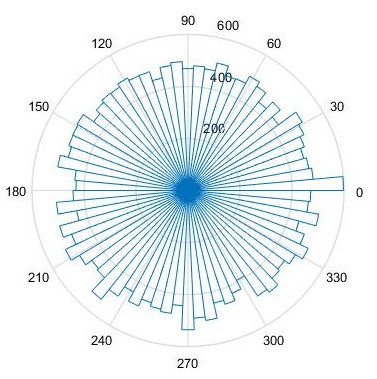
\includegraphics[scale=0.9]{Figuras/histograma_direccion.jpg}
\caption{Histograma polar de la dirección del viento}
Fuente: Elaboración Propia con datos de la OTS
\label{histograma_direccion}
\end{figure}

\begin{figure}[H]
\centering
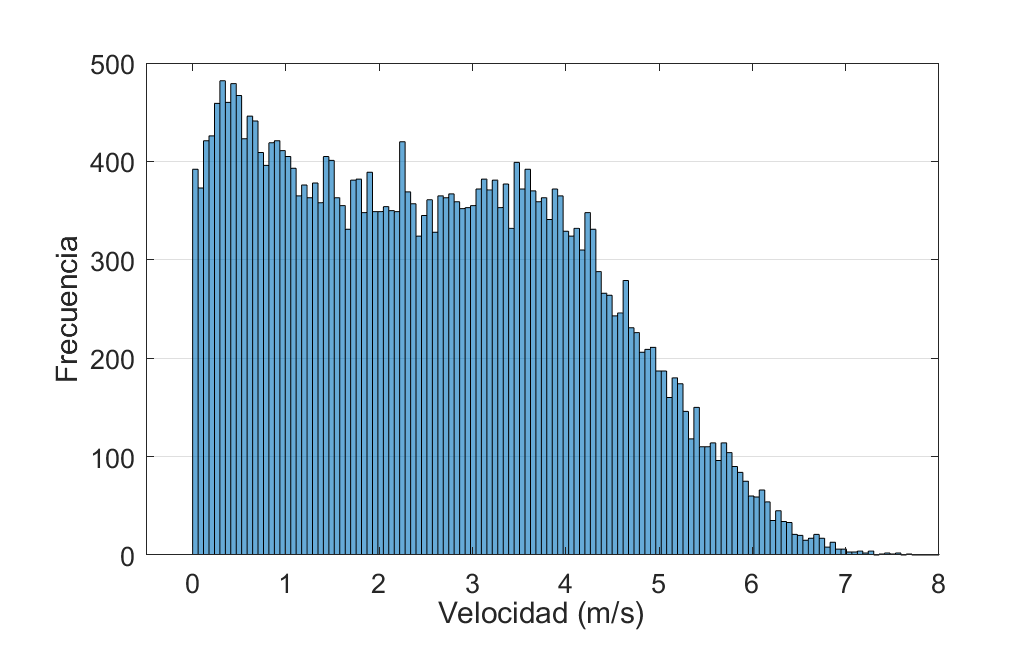
\includegraphics[scale=0.78]{Figuras/histograma_velocidad.eps}
\caption{Histograma de la velocidad del viento}
Fuente: Elaboración Propia con datos de la OTS
\label{histograma_velocidad}
\end{figure}

\begin{figure}[H]
\centering
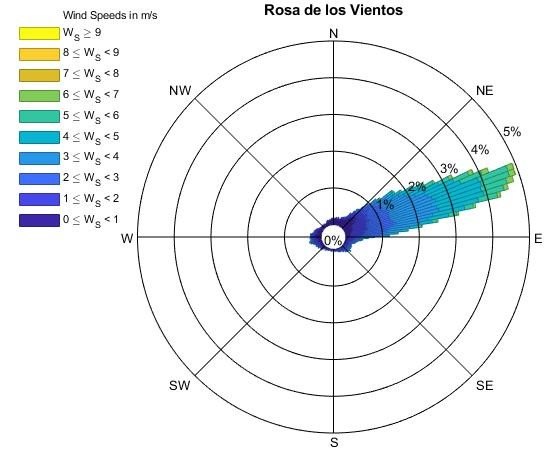
\includegraphics[scale=0.72]{Figuras/Rosa_de_los_vientos.jpg}
\caption{Histograma polar del vector viento}
Fuente: \cite{windrose} con datos de la OTS
\label{rosa_de_los_vientos}
\end{figure}

\subsection{Radiación Solar}

En la Tabla \ref{radiacion_met} se muestran los datos de radiación solar que llega a la Tierra recopilados por la estación meteorológica, en donde se tiene una resolución de \num{\pm\,1} \si{\watt/\square\meter} para los equipos de alta calidad y \num{\pm\,5}\si{\watt/\square\meter} para los de buena calidad; en cuanto a la exactitud las regulaciones de la OMM exigen \num{\pm2}\si{\percent} para la radiación global y de \num{\pm5}\si{\percent}  para la radiación neta. \cite{ots_manual}       

\begin{table}[H]
\centering
\caption{Datos de Radiación Solar entre el período del 1/6/2019 a 1/6/202 }
\label{radiacion_met}
\begin{tabular}{ccc}
\toprule
\textbf{Variable}     & \textbf{Promedio}          & \textbf{Máxima}          \\ \midrule
Radiación Solar \si{\watt/\square\meter} & \multicolumn{1}{c}{467,77} & \multicolumn{1}{c}{3361} \\ \bottomrule
\end{tabular}
\end{table}

\subsection{Humedad Relativa}

La resolución esperada de los datos para este rubro es de \SI{1}{\percent} y no más de \SI{3}{\percent} para el margen de error.\cite{ots_manual}

\begin{table}[H]
\centering
\caption{Datos de Humedad Relativa entre el período del 1/6/2019 a 1/6/202 }
\label{humedad_met}
\begin{tabular}{cccc}
\toprule
\textbf{Humedad Relativa (\si{\percent})} & \multicolumn{1}{l}{\textbf{Promedio}} & \multicolumn{1}{l}{\textbf{Máxima}} & \textbf{Mínima} \\ \midrule
Diurna                         & 63,58                                 & 98,70                               & 0,60            \\
Nocturna                       & 76,41                                 & 98,70                               & 0,51            \\ \bottomrule
\end{tabular}
\end{table}

\section{Esquema de Modelado}

La estrategia a seguir es muy similar a la utilizada para el radio transmisor, de hecho se basa en seguir el mismo esquema solamente que ampliado, consiste en tomar el modelo del radio y ampliarlo tomando en cuenta todas las condiciones termodinámicas que el radio enfrentará cuando este dentro de un gabinete en la ubicación antes descrita, y observar el comportamiento tanto del radio como de la estación y basados en estos datos obtenidos plantear una solución que se ajuste a esas condiciones operativas proyectadas.

Basado en el esquema mostrado en la Figura \ref{esquema_modelo_radio}, esta sección del proyecto consiste en ampliar el bloque referente a los \textit{Elementos Térmicos} tal y como se muestra en la Figura \ref{esquema modelo general}. Una de las suposiciones de este modelo es asumir que tanto el radio como el gabinete son dos esferas concéntricas una dentro de otra, de área superficial equivalente a sus respectivas configuraciones geométricas esto simplifica considerablemente los cálculos y procedimientos analíticos, principalmente para las estimaciones de la radiación, tal y como se vio en el marco teórico.

El objetivo es integrar el concepto de red generalizada visto en \cite{alfaro}; por otra parte en la literatura se observó que estos modos de abordar un problema de este tipo dan como resultado buenas aproximaciones en comparación de otros modelos más complejos.\cite{realtime}

\begin{figure}[H]
\centering
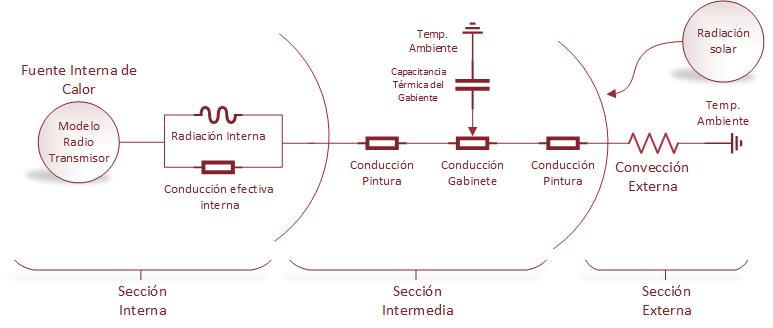
\includegraphics[scale=0.75]{Figuras/Esquema_de_Modelo_general.jpg}
\caption{Esquema de Modelo para la GRT}
Fuente: Elaboración Propia \label{esquema modelo general}
\end{figure}

\subsection{Consideraciones Generales de Simulación}

Por tratarse de una simulación termodinámica, para la resolución matemática de cada uno de los elementos involucrados se deben realizar suposiciones que permitan utilizar expresiones que dan como resultado los parámetros que se introducen dentro del software, el cual los unifica en un modelo que permite medir condiciones de flujo de calor y temperatura a través de sus diferentes secciones; dichas suposiciones se muestran a continuación

\begin{enumerate}
    \item Al igual que en el modelo del radio, se utilizarán los datos y parámetros de transmisión del experimento 2, y representar la condición más esforzada posible del radio, por la razones ya antes explicadas.
    \item Utilizar una configuración geométrica de dos esferas concéntricas, conlleva a que la fuente de calor (radio transmisor), también se considere con una posición central, esto es importante en el caso de la determinación del coeficiente de convección, debido a que los cálculos se realizaron considerando una placa en orientación vertical y no como una esfera a diferencia del resto de los cálculos; esto con el fin de determinar el coeficiente real de convección que se tendría dentro del gabinete.
    \item En las instancias en que se evalúen las propiedades del aire, se asume que el mismo se comporta como gas ideal.
    \item Para el caso de la radiación:
    \begin{itemize}
        \item Las superficies son opacas, difusas o grises, lo que implica que son emisoras y reflectoras difusas. 
        \item Las superficies son emisoras difusas con una emisividad igual al valor en la dirección normal.
        \item Sus propiedades relativas a la radiación son independientes de la longitud de onda.
        \item Cada superficie del recinto es isoterma y tanto la radiación entrante como saliente son uniformes sobre cada superficie.
        \end{itemize}
\end{enumerate}

\section{Parámetros de Simulación}

Considerando la literatura y las ecuaciones mostradas en el marco teórico a continuación se muestran los resultado de los cálculos para los parámetros de simulación a manera de tablas resumen donde se muestran los resultados del procedimiento planteado en la teoría. Para todos los casos las propiedades del aire fueron evaluadas a la presión atmosférica

\subsection{Determinación del coeficiente de convección del módulo de potencia}

\begin{table}[H]
\centering
\caption{Resultados del cálculo para la determinación del coeficiente de convección real}
\label{calculo1}
\begin{tabular}{cccc}
\toprule
\textbf{Variable} & \textbf{Valor} & \textbf{Unidad}      & \textbf{Ecuación utilizada} \\ \midrule
$T_{s}$          & 75             & \si{\celsius}          & Parámetro de diseño         \\
$T_{\infty}$ & 30 & \si{\celsius} & Parámetro de diseño \\
$A_{modulo}$ & \num{8,964e-4} & \si{\square\meter} & Parámetro constructivo \\
$T_{f}$ & 325,65 & \si{\kelvin} & \ref{tf} \\
$Ra_{L}$ & 58456,189 & $N/A$  & \ref{ra1} \\
$Nu$ & 8,079 & $N/A$& \ref{nu1}  \\
$h$ & 5,515 & \si{\watt/\square\meter\cdot\celsius} & \ref{h1} \\ \bottomrule
\end{tabular}
\end{table}

En la Tabla \ref{calculo1} se muestra la temperatura $T_{f}$ a la cual fue evaluada las propiedades del aire. Por otro lado el resultado para el coeficiente de convección difiere tan solo en un \SI{9,34}{\percent} del valor utilizado como estimación para el modelo del radio. 

\subsection{Parámetros del aire interno del gabinete}

Para esta sección el cálculo se divide en dos partes, una es el cálculo del coeficiente de conducción efectiva para el aire y la otra es la determinación de los parámetros de radiación entre dos placas. Ambos parámetros junto con el modelo del radio representan la sección interna de la estación (Figura \ref{esquema modelo general}).

\textbf{Coeficiente efectivo del aire:}

\begin{table}[H]
\centering
\caption{Coeficiente efectivo de conducción para el aire}
\label{calculo2}
\begin{tabular}{cccc}
\toprule
\textbf{Variable} & \textbf{Valor} & \textbf{Unidad}  & \textbf{Ecuación utilizada} \\ \midrule
$T_{s}$          & 75             & \si{\celsius}     & Parámetro de diseño         \\
$T_{\infty}$ & 30 & \si{\celsius} & Parámetro de diseño \\
$T_{prom}$ & 53,725 & \si{\celsius}& \ref{tprom} \\
$Lc$ & 0,521 & \si{\meter}  & \ref{lc}\\
$F_{esf}$ &  $2,89\times 10^{-5}$ & $N/A$ & \ref{fesf} \\
$Ra_{L}$ & 410450834,398  & $N/A$ & \ref{ra1}  \\
$Nu$ & 8,079 & $N/A$ & \ref{nu1}  \\
$k_{ef}$ & 0,2208 & \si{\watt/\meter\cdot\celsius} & \ref{h1}\\
\bottomrule
\end{tabular}
\end{table}

Si se compara el coeficiente de conducción del aire evaluado a la temperatura $T_{prom}$ contra el coeficiente $k_{ef}$ se tiene que este último es 8 veces más grande, de ahí radica la importancia de este cálculo para recintos cerrados.

\textbf{Radiación interna del recinto:} El software para realizar el cálculo de la radiación entre dos placas o paredes utiliza lo que denomina un factor de radiación, que se denominará en este proyecto como $k_{rad}$, el cual depende en cierta manera de la configuración geométrica de las placas; además este factor de radiación es equivalente a tomar la Ecuación \ref{radint} y reducirla a contener parte de sus términos dentro del factor antes mencionado, tal y como se muestra a continuación.

\begin{equation}\label{kradiacion}
    k_{rad}=\frac{\sigma }{\frac{1}{\varepsilon _{1}}+\frac{1-\varepsilon _{2}}{\varepsilon _{2}}\cdot \left | \frac{r_{1}}{r_{2}} \right |^{2}}\;\;(\si{\watt/\square\meter\cdot\kelvin\tothe{4}}) 
\end{equation}

En la tabla se muestran los valores de emisividad correspondientes para cada caso, cabe aclarar que en este cálculo se está considerando la radiación existente entre la superficie del módulo de potencia (considerada como una esfera) y la superficie interna del gabinete, la cual es la capa de pintura, por lo que el dato de emisividad debía ser justamente del tipo de pintura.

Debido a la dificultad de obtener un dato de emisividad para la pintura en específico que utiliza el gabinete, por lo que se utilizó el valor de pinturas con características similares y se habla de similares ya que la literatura no es concluyente respecto a si el color influye en el valor de emisividad; hay fabricantes que asocian un valor de emisividad a sus pinturas obtenidos de manera experimental, mientras que existen estudios que indican que el color de la pintura no influye en dicho factor, sino más bien la forma de aplicación, el acabado y la composición de la misma. \cite{flir},\cite{indecolor} 

\begin{table}[H]
\centering
\caption{Parámetros para el factor de radiación}
\label{calculo3}
\begin{tabular}{cccc}
\toprule
\textbf{Variable}   & \textbf{Valor} & \textbf{Unidad} & \textbf{Ecuación utilizada} \\ \midrule
$\varepsilon _{1}$ & 0,1            & $N/A$           & Parámetro constructivo      \\
$\varepsilon _{2}$ & 0,9            & $N/A$           & Parámetro constructivo      \\
$r_{1}$ & 0,0084 & \si{\meter}& $N/A$           \\
$r_{2}$  & 0,2688 & \si{\meter} & $N/A$ 
\\
$k_{rad}$ & \num{5,6699e-9} & \si{\watt/\square\meter\cdot\kelvin\tothe{4}}& \ref{kradiacion}\\
\bottomrule
\end{tabular}
\end{table}

El valor de emisivilidad para el módulo de potencia, es el de un metal pulido y los valores $r_{1}$ y $r_{2}$ son los correspondientes al radio de una esfera de un área superficial equivalente al del módulo y al gabinete respectivamente.  

\subsection{Parámetros del Gabinete}

Para la determinación de estos parámetros, se hizo uso de la herramienta de modelado CAD 3D \textit{fusion 360} para lograr determinar características físicas que no eran mencionadas dentro de las especificaciones del fabricante; el cual tampoco es muy específico en cuanto al material del gabinete, salvo de indicar que se trata de acero, por lo que se asumió para los cálculos un acero AISI 1010 y sus propiedades se obtuvieron de. \cite{cengel}

\begin{table}[H]
\centering
\caption{Características para el gabinete}
\label{calculo4}
\begin{tabular}{cccc}
\toprule
\textbf{Variable} & \textbf{Valor} & \textbf{Unidad} & \textbf{Ecuación utilizada} \\ \midrule
$A_{s}$ & 1,03643 & \si{\square\meter} & Parámetro constructivo      \\
$m$ & \num{\sim10,48} & \si{\kilogram}  & Parámetro constructivo\\
$C_{p}$ & 434 & \si{\joule/\kilogram\cdot\kelvin}& Dato de Tabla
\\
$k$ & 63,9 & \si{\watt/\meter\cdot\kelvin} & Dato de Tabla
\\
\bottomrule
\end{tabular}
\end{table}

Esta sección consta de tres elementos que se pueden agrupar en dos; uno es la determinación de la resistencia térmica conductiva tanto de la pintura como del gabinete y la determinación de la capacidad calorífica del gabinete, es decir su capacitancia térmica o capacidad de almacenar energía calórica. Estos tres elementos componen la sección intermedia de la Figura \ref{esquema modelo general}.

\textbf{Resistencia térmica del gabinete y pintura:} Una forma de estimar la transferencia de calor a través de una pared de espesor $L$, es utilizando la analogía eléctrica de la resistencia y observar esta pared como un elemento que se opone al flujo de calor de modo que se puede obtener una expresión como la siguiente para determinar la resistencia térmica. \cite{cengel}

\begin{equation}\label{resistencia}
    R_{cond}=\frac{r_{2}-r_{1}}{4\pi  r_{1}r_{2}\cdot  k}\;\;(\si{\celsius/\watt})
\end{equation}
 
Donde: 

\begin{itemize}
    \item $r_{1}$ es el diámetro interno de pared (\si{\meter})
    \item $r_{2}$ es el diámetro externo de pared (\si{\meter})
    \item $k$ es el coeficiente de conductividad térmica (\si{\watt/\meter\cdot\kelvin})
\end{itemize}

Los valores $r_{1}$ y $r_{1}$ se pueden determinar fácilmente con el espesor de lámina del gabinete y del cálculo de radio equivalente para el área superficial del gabinete. Tomando eso en consideración en la Tabla \ref{calculo5} se muestran los resultados obtenidos para  las resistencias térmicas.\cite{cengel}

\begin{table}[H]
\centering
\caption{Resistencias térmicas para la sección intermedia}
\label{calculo5}
\begin{tabular}{cccc}
\toprule
\textbf{Variable} & \textbf{Valor}                                        & \textbf{Unidad} & \textbf{Ecuación utilizada}        \\ \midrule
$R_{gabinete}$   & \num{1,886e-5} & \si{\celsius/\watt}  & \ref{resistencia} \\
$R_{pintura}$    & 0,1707  & \si{\celsius/\watt}  & \ref{resistencia} \\ \bottomrule
\end{tabular}
\end{table}

\textbf{Capacitancia térmica del gabinete:} Este bloque el software lo representa como la capacidad del cuerpo para almacenar energía en forma de calor considera su masa y calor específico, el cálculo lo realiza el software mediante la siguiente ecuación. Los valores asociados a la Ecuación \ref{thermal mass} se encuentran especificados en la Tabla \ref{calculo4}.

\begin{equation}\label{thermal mass}
    Q=c\cdot m\frac{dT}{dt}\;\;(\si{\watt})
\end{equation}

Donde:

\begin{itemize}
    \item $c$ es el calor específico (\si{\joule/\kilogram\cdot\kelvin})
    \item $m$ es la masa (\si{\kilogram})
\end{itemize}

\subsection{Parámetros externos}

Como su nombre lo indica, corresponde a los parámetros correspondientes a la sección externa del esquema de modelo, compuesta por los elementos que describen el coeficiente de convección externa y la estimación de la radiación entrante en el gabinete.

\textbf{Coeficiente de convección externa:} Para este cálculo se utilizaron los datos de velocidad del viento de la Tabla \ref{viento_met}. Además se establecen los parámetros de temperatura del aire y temperatura promedio externa del aire para la evaluación de las propiendas del aire.

\begin{table}[H]
\centering
\caption{Cálculos del coeficiente de convección externa}
\label{calculo6}
\begin{tabular}{cccc}
\toprule
\textbf{Variable} & \textbf{Valor}  & \textbf{Unidad}      & \textbf{Ecuación utilizada} \\ \midrule
$T_{aire}$ & 30,45  & \si{\celsius} & Parámetro ambiental \\
$T_{prom}$ & 29,97 & \si{\celsius} & Parámetro ambiental
\\
$Nu$ & \num{1,886e-5} & $N/A$ & \ref{nu2} \\
$Re$ & 0,1707 & $N/A$ & \ref{re2}\\
$h$ & 14,5728 & \si{\watt/\square\meter\cdot\celsius} & \ref{hext} \\
\bottomrule
\end{tabular}
\end{table}

\textbf{Determinación Radiación Solar:} En cuanto a la radiación, el modelo contempla este dato como una fuente de calor aplicada a la mitad del área de una esfera, ya que bajo esta simplificación la radiación sin importar la posición del sol siempre irradiará la mitad de la esfera, por lo que quedaría considerar simplemente el momento del día en el cual la radiación es más intensa, y esto es de esperarse en horas del medio día según los datos de la OTS.

Para determinar la magnitud de esta fuente de calor existían dos posibilidades: una consiste en utilizar los datos meteorológicos, y el otro en realizar los cálculos demostrados en la teoría apoyados con la utilización de un algoritmo de posición solar implementado por la National Renewable Energy Laboratory (NREL) el cual permite considerar la ubicación exacta del lugar, parámetros de presión atmosférica, altitud, incluso realizar una estimación para una fecha y hora en específico \cite{spa} . En la Tabla \ref{comparacion radiacion} se muestra una comparación para la fecha y hora indicadas entre los datos meteorológicos y los resultados obtenidos de los cálculos realizados con base en la teoría y con el soporte del algoritmo.

\begin{table}[H]
\centering
\caption{Comparativa entre las estimaciones para la radiación solar}
\label{comparacion radiacion}
\begin{tabular}{ccc}
\toprule
\textbf{Herramienta} & \textbf{Valor (\si{\watt/\square\meter})} & \textbf{Fecha y hora de evaluación}       \\ \midrule
Algoritmo & 1036,4 & \multirow{2}{*}{4 de mayo de 2020 a las 12:15 pm} \\
Datos Meteorológicos & 1054 &             \\
\bottomrule
\end{tabular}
\end{table}

La diferencia entre los dos métodos para esta fecha y hora en específico es de apenas \SI{1,68}{\percent}, sin embargo cuando se trata de cálculos de radiación solar se debe tener especial cuidado, ya que el hecho de que exista una nube en el momento de la medición, para el caso del dato meteorológico, cambia completamente el dato mostrado y la variación podría ser significativa. Es por esta razón que se decide implementar el cálculo de radiación solar mediante el algoritmo, y utilizar el valor mostrado en la Tabla \ref{comparacion radiacion}, ya que este permite realizar estimación de radiación para fechas especificas y sobre superficies con diferentes ángulos de inclinación en caso de ser necesario, lo cual le atribuye la ventaja de  poderse utilizar para modelos de estaciones en otras ubicaciones geográficas también.

Para el caso especifico de la GRT en Palo Verde se recomienda, siempre y cuando se pueda, realizar la comparación entre los dos métodos en la evaluación de fechas pasadas de manera que se tenga una estimación más fiable de la radiación, principalmente su alta desviación estándar en las mediciones. En el Apéndice se muestra el dato de la OTS usado en la Tabla \ref{comparacion radiacion}.

\textbf{Humedad:} Como es de esperar los valores de humedad relativa durante el día son elevados, alrededor de \SI{70,32}{\percent} promedio durante el período evaluado para los demás parámetros. Al utilizar la Ecuación \ref{calculo td} para estimar la posibilidad de condensación en el gabinete, se observó que las horas nocturnas presentaban el mayor riesgo, ya que en ocasiones tenían valores de temperatura de rocío cercanos a la temperatura ambiente. Sin embargo, al igual que en el caso de la radiación, los parámetros de humedad relativa tienen una alta variabilidad en el tiempo más aún que depende de factores como la temperatura ambiente y la presión atmosférica.


\section{Resultados de Simulación}

Para todas la simulaciones realizadas, se partía de la suposición de un día claro al medio día, con valores promedio de temperatura y velocidad del viento diurnas constantes para un lapso de \SI{850}{\second}. Para el caso de los valores de temperatura mostrados en las Figura \ref{gabinete t}, se muestran las temperaturas obtenidas de la simulación en contraste con los datos de temperatura real, a manera de punto de referencia para la comparación. Por otra parte, en la Figura \ref{gabinete q} se observa el flujo de calor entregado por el radio hacia el gabinete. En el Anexo \ref{anexo10} se muestra el algoritmo construido para la obtención de los resultados.

\begin{figure}[H]
\centering
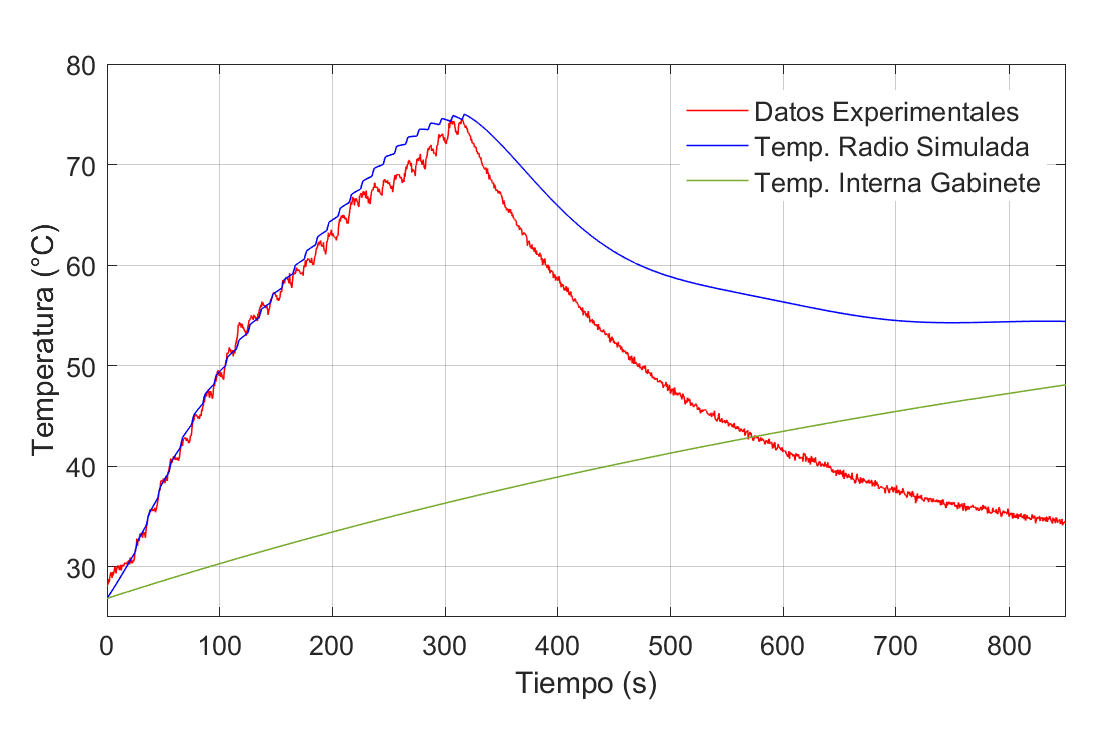
\includegraphics[scale=0.7]{Figuras/Gabinete_T.eps}
\caption{Gráfica Temperaturas vs tiempo}
Fuente: Elaboración Propia \label{gabinete t}
\end{figure}

\begin{figure}[H]
\centering
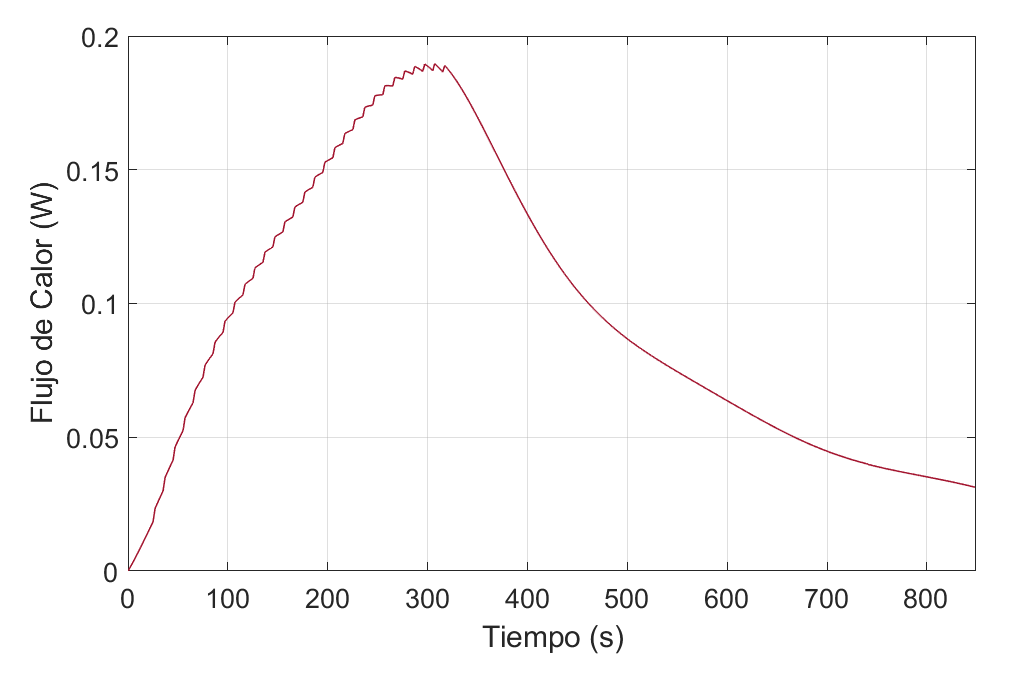
\includegraphics[scale=0.75]{Figuras/Gabinete_Q.eps}
\caption{Gráfica de Flujo de calor vs tiempo}
Fuente: Elaboración Propia \label{gabinete q}
\end{figure}

\subsection{Análisis de Resultados}

De los datos obtenidos se extraen las siguientes observaciones.

\begin{enumerate}
    \item En la Figura \ref{gabinete t} se observa como el perfil de temperatura para el radio, se ve afectado luego de que finaliza la transmisión, donde la temperatura de estabilización se alcanza aproximadamente a los \SI{55}{\celsius}; en este punto es donde la radiación solar afecta el módulo de potencia en el caso de que el mismo no posea un disipador.
    \item La temperatura interna del gabinete de la Figura \ref{gabinete t} representa en el modelo la temperatura entre el aire interno del gabinete y la capa interna de pintura del mismo. De igual manera que para el módulo de potencia, presenta una elevación de temperatura a una tasa aproximada de \SI{1,5}{\celsius/\min} donde la temperatura de equilibrio térmico de la estación estaría aproximadamente a los \SI{55}{\celsius}.
    \item Si bien es cierto la temperaturas observadas se acercan al punto de operación máximo para el radio transmisor, se debe considerar que el flujo de calor por radiación simulado es constante, lo cual no sucede en la realidad, como ya se mencionó los datos observados de radiación de la estación meteorológica indican una gran variabilidad de este valor en intervalos incluso de \SI{15}{\min} y con desviaciones estándar muy elevadas sin embargo, el valor de radiación utilizado representa un valor promedio de radiación para la zona, por lo que sus efectos en la GRT no deben ser despreciados.
    \item Como era de esperarse el flujo de calor por parte del radio hacia el gabinete se observa que no varia respecto al modelo del radio, salvo que en esta ocasión el valor es positivo porque en el contexto del modelo el sistema es el gabinete como tal por lo tanto la energía es entregada por el radio hacia el sistema.
\end{enumerate}

